\chapter{Dokumentation for SPI forbindelse imellem Devit8000 og PSoC}

\section{Indleding}
I wineprep projektet skal der bruges en linux platform, som i dette projekt består af et devkit8000 hvorpå der er installeret distributionen Ångstöm. 
Denne skal tage imod input fra brugeren af systemet via en grafisk brugergrænseflade og omskrive disse til kommandoer, som sendes til PSoC. Desuden
vil PSoC sende status beskeder tilbage til Devkittet. 
Der vil i projektet indgå en PSoC, som står for kommunikationen med Devkit8000 samt for nogle af systemets motorer og sensorer.
Men på grund af et begrænset antal GPIO pinde på PSoC, vil det blive nødvendigt med to ekstra PSoC, som kan tage sig af kommunikationen med de 
øvrige motorer og sensorer i systemet. Der vil derfor blive lavet en forbindelse mellem de tre PSoC enheder. Der vil i denne documentation blive 
refereret til disse PSoC enheder som PSoC1 (forbindes til Devkit), PSoC2(forbindes til PSoC1) og PSoC3(forbindes til PSoC1). 
Ovenstående taget i betragtning vil det blive nødvendigt at etableres en tovejsforbindelse imellem devkit8000 og PSoC1, samt en tovejsforbindelse imellem 
PSoC1 og PSoC2, samt PSoC1 og PSoC3. 

Dette kan gøres på flere forskellige måder, f.eks. med en UART protokol som på tidligere semester projekter. Der er i fagene HAL og GFV på 3. semester 
blevet arbejdet en del med de to serielle dataforbindelses standarter I2C og SPI, og det vil derfor være nærliggende at benytte en af disse to. 
Det er fra gruppens side, og med opfordring fra vejleder blevet besluttet at SPI vil blive benyttet i dette projekt til forbindelsen imellem Devkit og 
PSoC. Grunden til dette valg er mest af alt bekvæmmelighed, da der allerede er arbejdet med SPI drivere til Linux og PSoC i tidligere laboratorie øvelser.   

\section{Design og implementering}
SPI er en synkron dataopførselsmetode, hvor to enheder indgår i et master-slave forhold, og hvor data sendes og modtages mellem de to enheder på
samme tid med klokken som "taktstok". For mere information omkring SPI protokollen henvises til bilag(*referance til SPI protokollen).
Devkit8000 vil i dette tilfælde udfører rollen som master i forbindelsen til PSoC1, hvilket også betyder at det er denne som står for at starte 
dataoverførelsen mellem de to enheder. Derudover vil PSoC1 fungere som master i forbindelsen til PSoC2 og PSoC3. 

\begin{figure}[H]
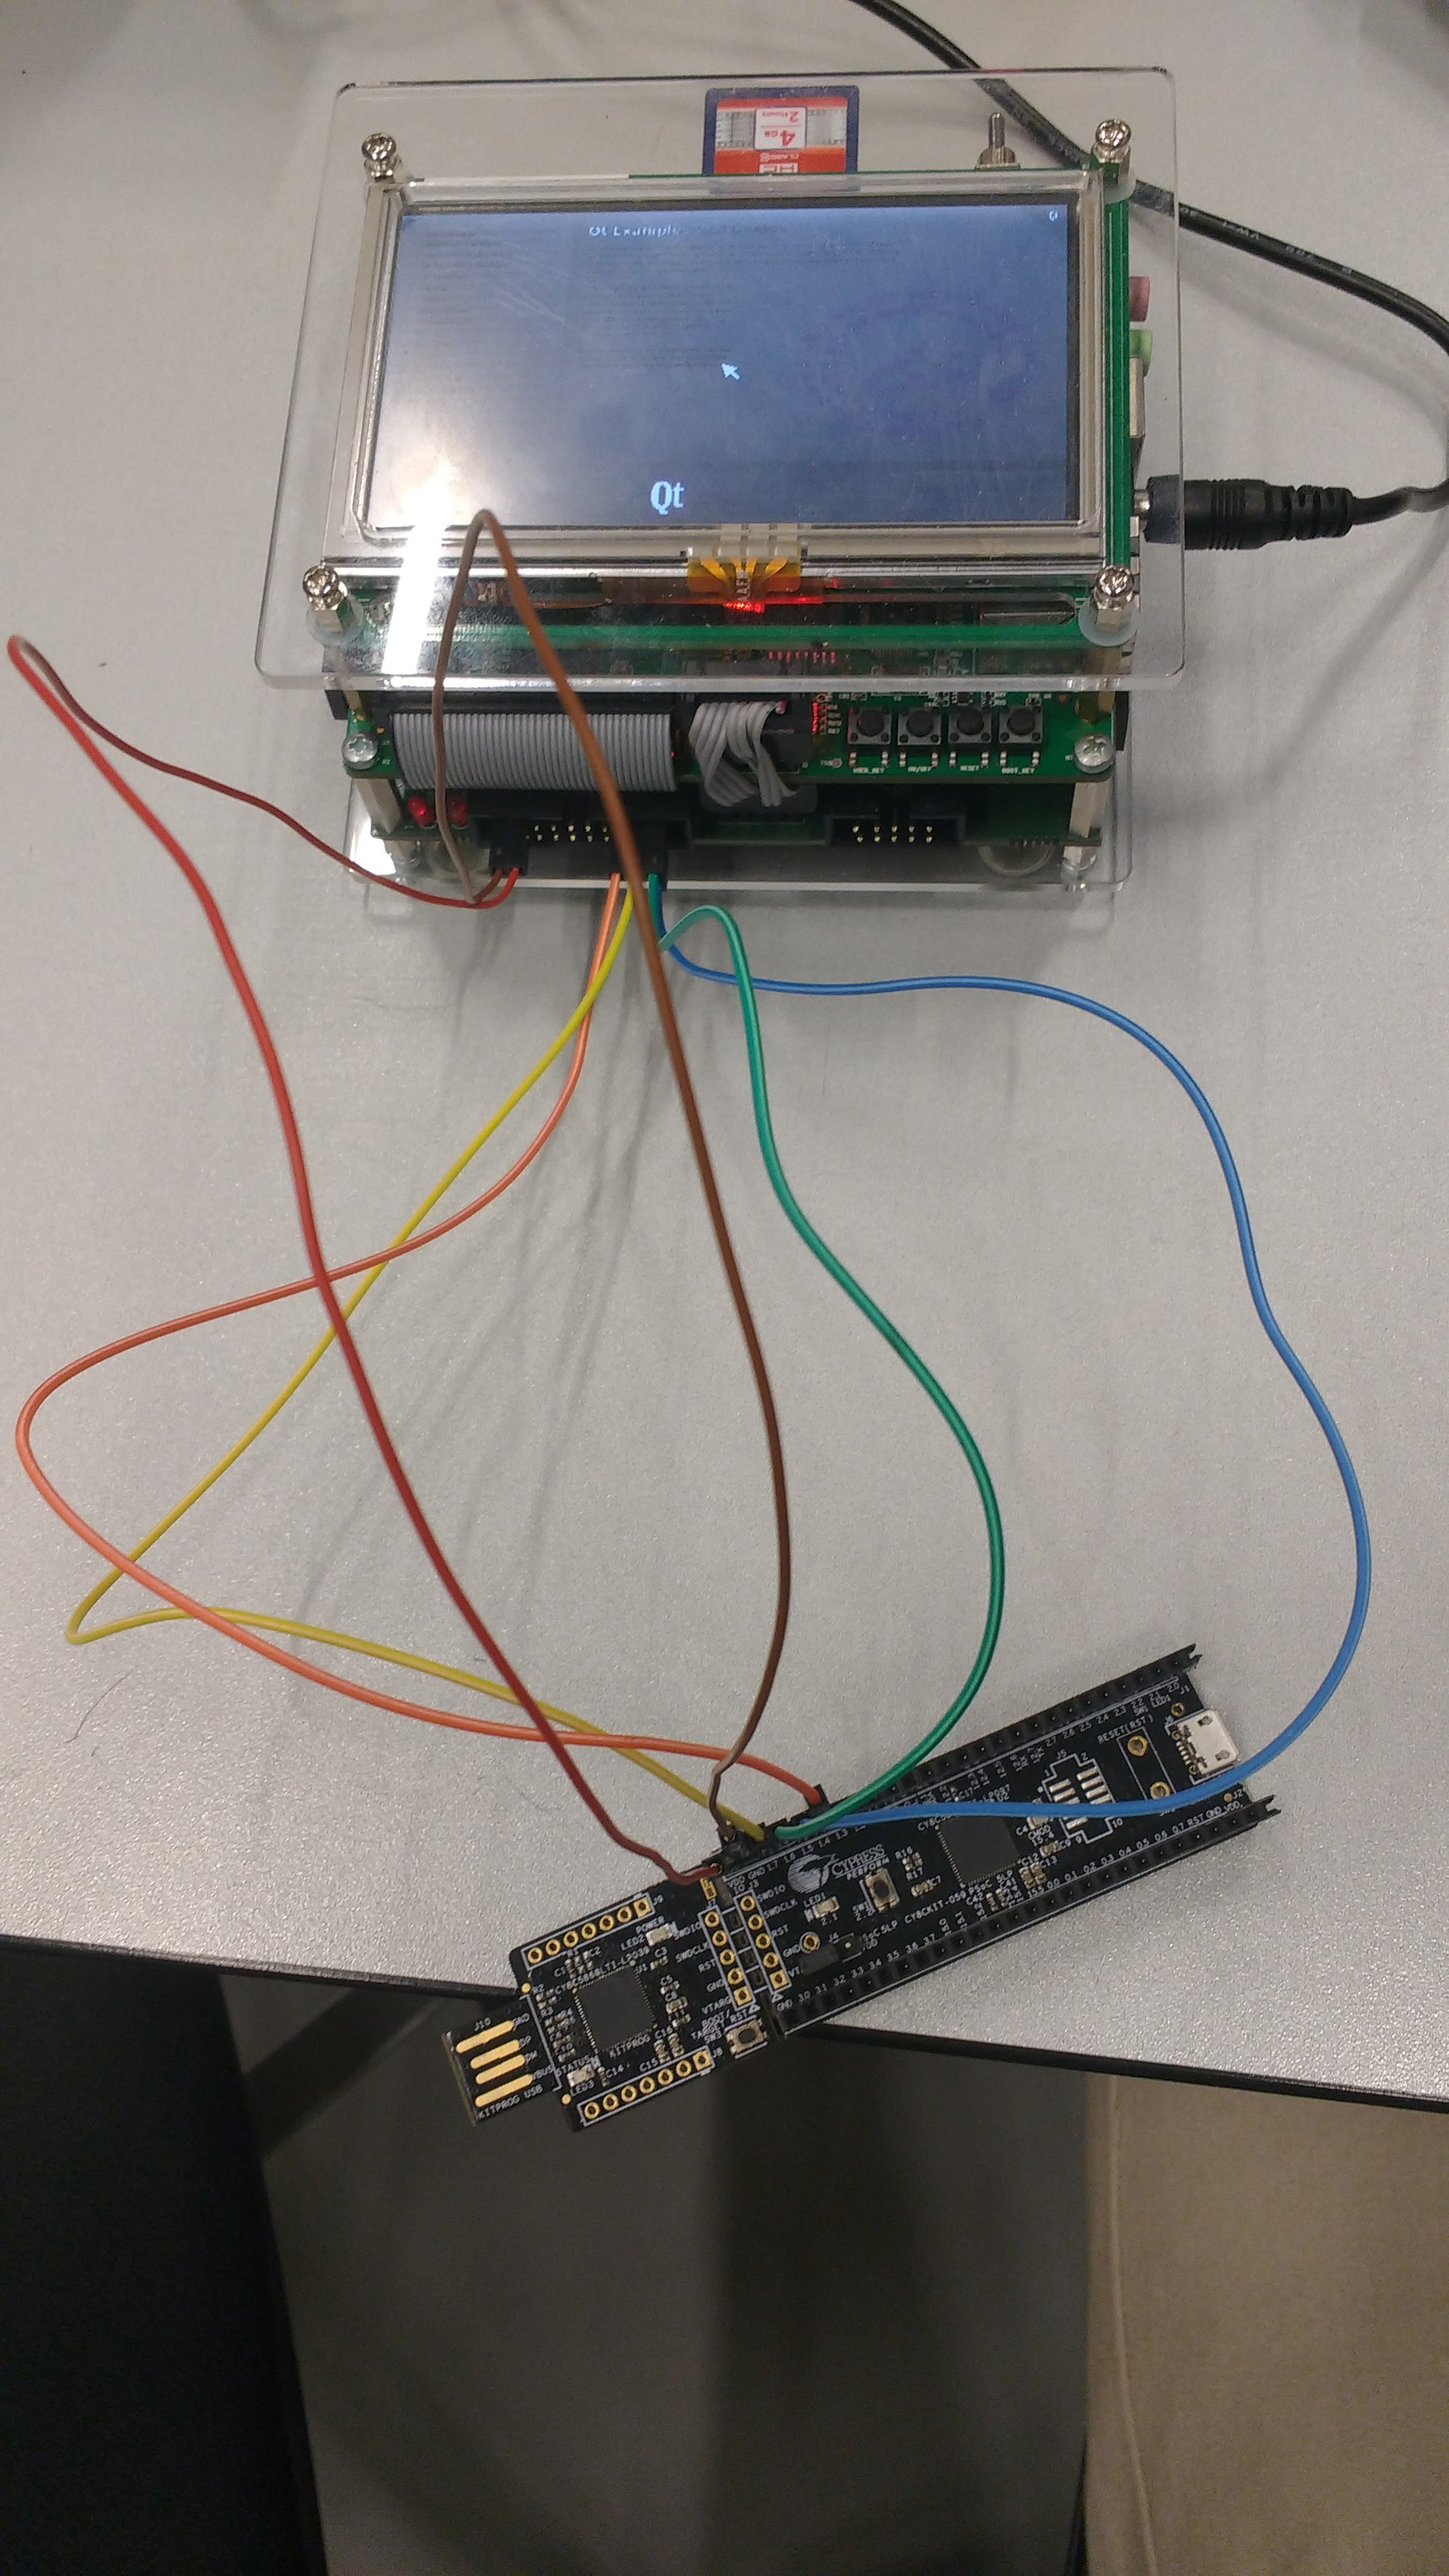
\includegraphics[scale=0.15]{Screenshots/Realisering_devkit_psoc}
\caption{Realisering af Devkit8000-PSoC SPI forbindelse}
\end{figure}

SPI undersøttes naturligvis af Devkit8000, men for at kunne etablere forbindelsen til PSoC1 skal den nødvendige SPI driver skrives til Linux. 
Denne driver indeholder blandt andet den korrekte opsætningen for forbindelsen, samt implementeringen af SPI metoderne til at sende/modtage data.
Der skal også skrives en character device driver, der gør det muligt for et program i userspace at tilgå SPI driveren. Der laves også en hotplug driver 
der gør det muligt at indsætte PSoC i runtime. For mere information omkring implementeringen af denne driver, samt eksempel på dens anvendelse henvises der til HAL 
øvelse 6 i bilag. 
Vi har i dette projekt anvendt den SPI driver som er blevet udleveret på redmine i faget HAL. Så SPI driver modulerne indsættes blot på devkit8000, og der 
laves de nødvendige device noder. Disse noder er nødvendige for at kunne kommunikere melle user- og kernelspace. 

\begin{figure}[H]
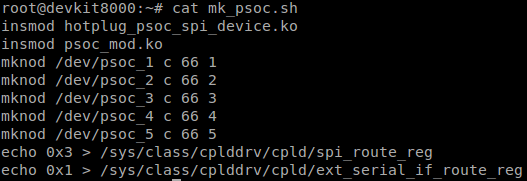
\includegraphics[scale=0.9]{Screenshots/Devkit_cat_mk_psoc}
\caption{Indsættelse af moduler i Linux kernen og oprettelse af device noder}
\end{figure}

De tre PSoC enheder skal ligesom Devkit også have implementetet software, der kan håndtere SPI forbindelsen, og reagere
på den ønskede måde når der modtages data. Denne software skrives med værktøjet PSoC-creator, som via et simpelt drag-and-drop interface, gør det
nemt at konfigurere SPI. Selve SPI driveren skal derfor ikke skrives, men der skal laves en source fil hvori det er muligt at kalde metoder til
styring af SPI, håndtere RX interrupts og anvende den modtagne data til at udføre forskellige opgaver for systemet.

\begin{figure}[H]
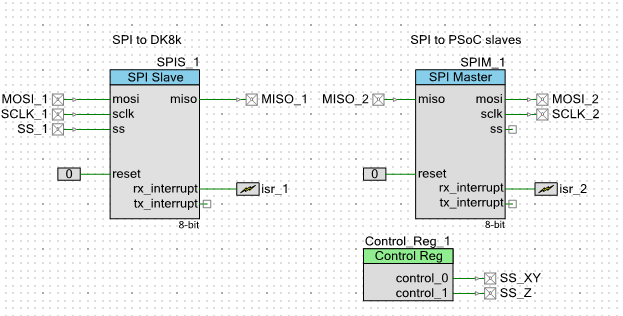
\includegraphics[scale=0.8]{Screenshots/PSOC_opstilling_spi}
\caption{Topdesign for PSoC1}
\end{figure}

PSoC1 skal have både et SPI-master(SPIM) og et SPI-slave(SPIS) modul i PSoC-creator. Der ønskes et interrupt ved RX på SPIS, da slaven skal reagere
hver gang der modtages data fra master, hvorefter der skal skrives tilbage, og udføres en opgave. Dette vil blive håndteret i main af en switch 
implementation, der kaldes hver gang RX interruptet flaget går højt. SPI driveren på Devit8000 er opsat således at der sendes 16 bits til PSoC1.
Af disse er de første 8 bit tiltænkt adresse- og kommandobits, og de næste 8 bit er selve data. Der vil i main først blive switched på adresse bits,
disse fortæller hvilken overordnet case der benyttes. Kommandobits indikerer om der ønskes data læst tilbage fra PSoC1, eller om det blot er 
tilstækkeligt at PSoC1 behandler den modtagne data, og sender nogle 0 værdier tilbage. Der vil vi inde i switchen være mulighed for at PSoC1 giver 
data videre til PSoC2 og PSoC3 i tilfælde, hvor den ikke selv kan udføre den pågældende opgave. Her vil PSoC1 bruge metoder fra SPIM, og fungere som master 
i forhold til PSoC2 og PSoC3. 

\begin{figure}[H]
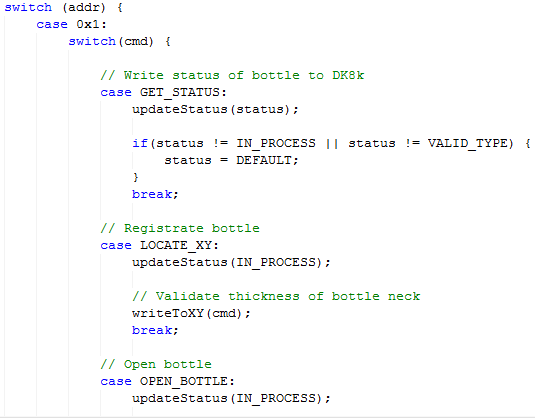
\includegraphics[scale=0.9]{Screenshots/PSOC_switch}
\caption{Eksempel på en switch statement i PSoC koden}
\end{figure}

Topdesign og koden for PSoC2 og PSoC3 vil blive implementeret næsten på samme måde som PSoC1, hvor der implenteres et RX interrupt og en switch som 
behandler den modtagne data. De to slave PSoC enheder vil dog kun have et SPIS modul implementeret, og derfor have færre switch cases.
Der bruges en 8bit kommando til at sende data til PSoC2 og PSoC3, det er denne kommando, som bliver switched på.  
\begin{figure}[H]
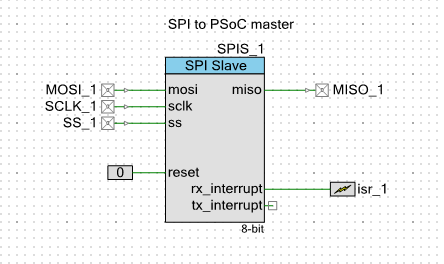
\includegraphics{Screenshots/PSOC_topdesign_SPIS}
\caption{Topdesing for PSoC2 og PSoC3}
\end{figure}

\begin{figure}[H]
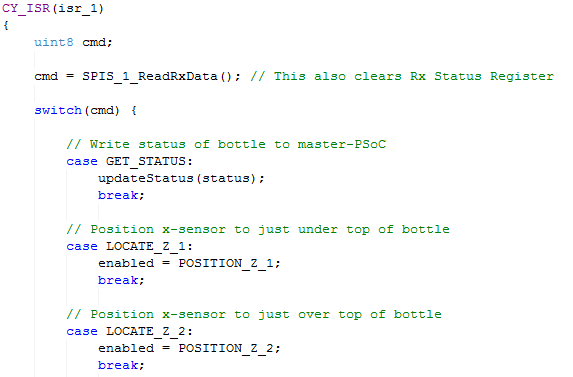
\includegraphics[scale=0.9]{Screenshots/PSOC_switch_slave}
\caption{Eksempel på switch cases for PSoC2 og PSoC3}
\end{figure}     
 
\section{Test}

\subsection{Test af SPI forbindelse imellem Devit8000 og PSoC1}

Testen for SPI forbindelsen imellem Devkit8000 og PSoC1 foretages med analog discovery, hvor der måles på SS, CLCK, og henholdsvis MISO og MOSI.

\begin{figure}[H]
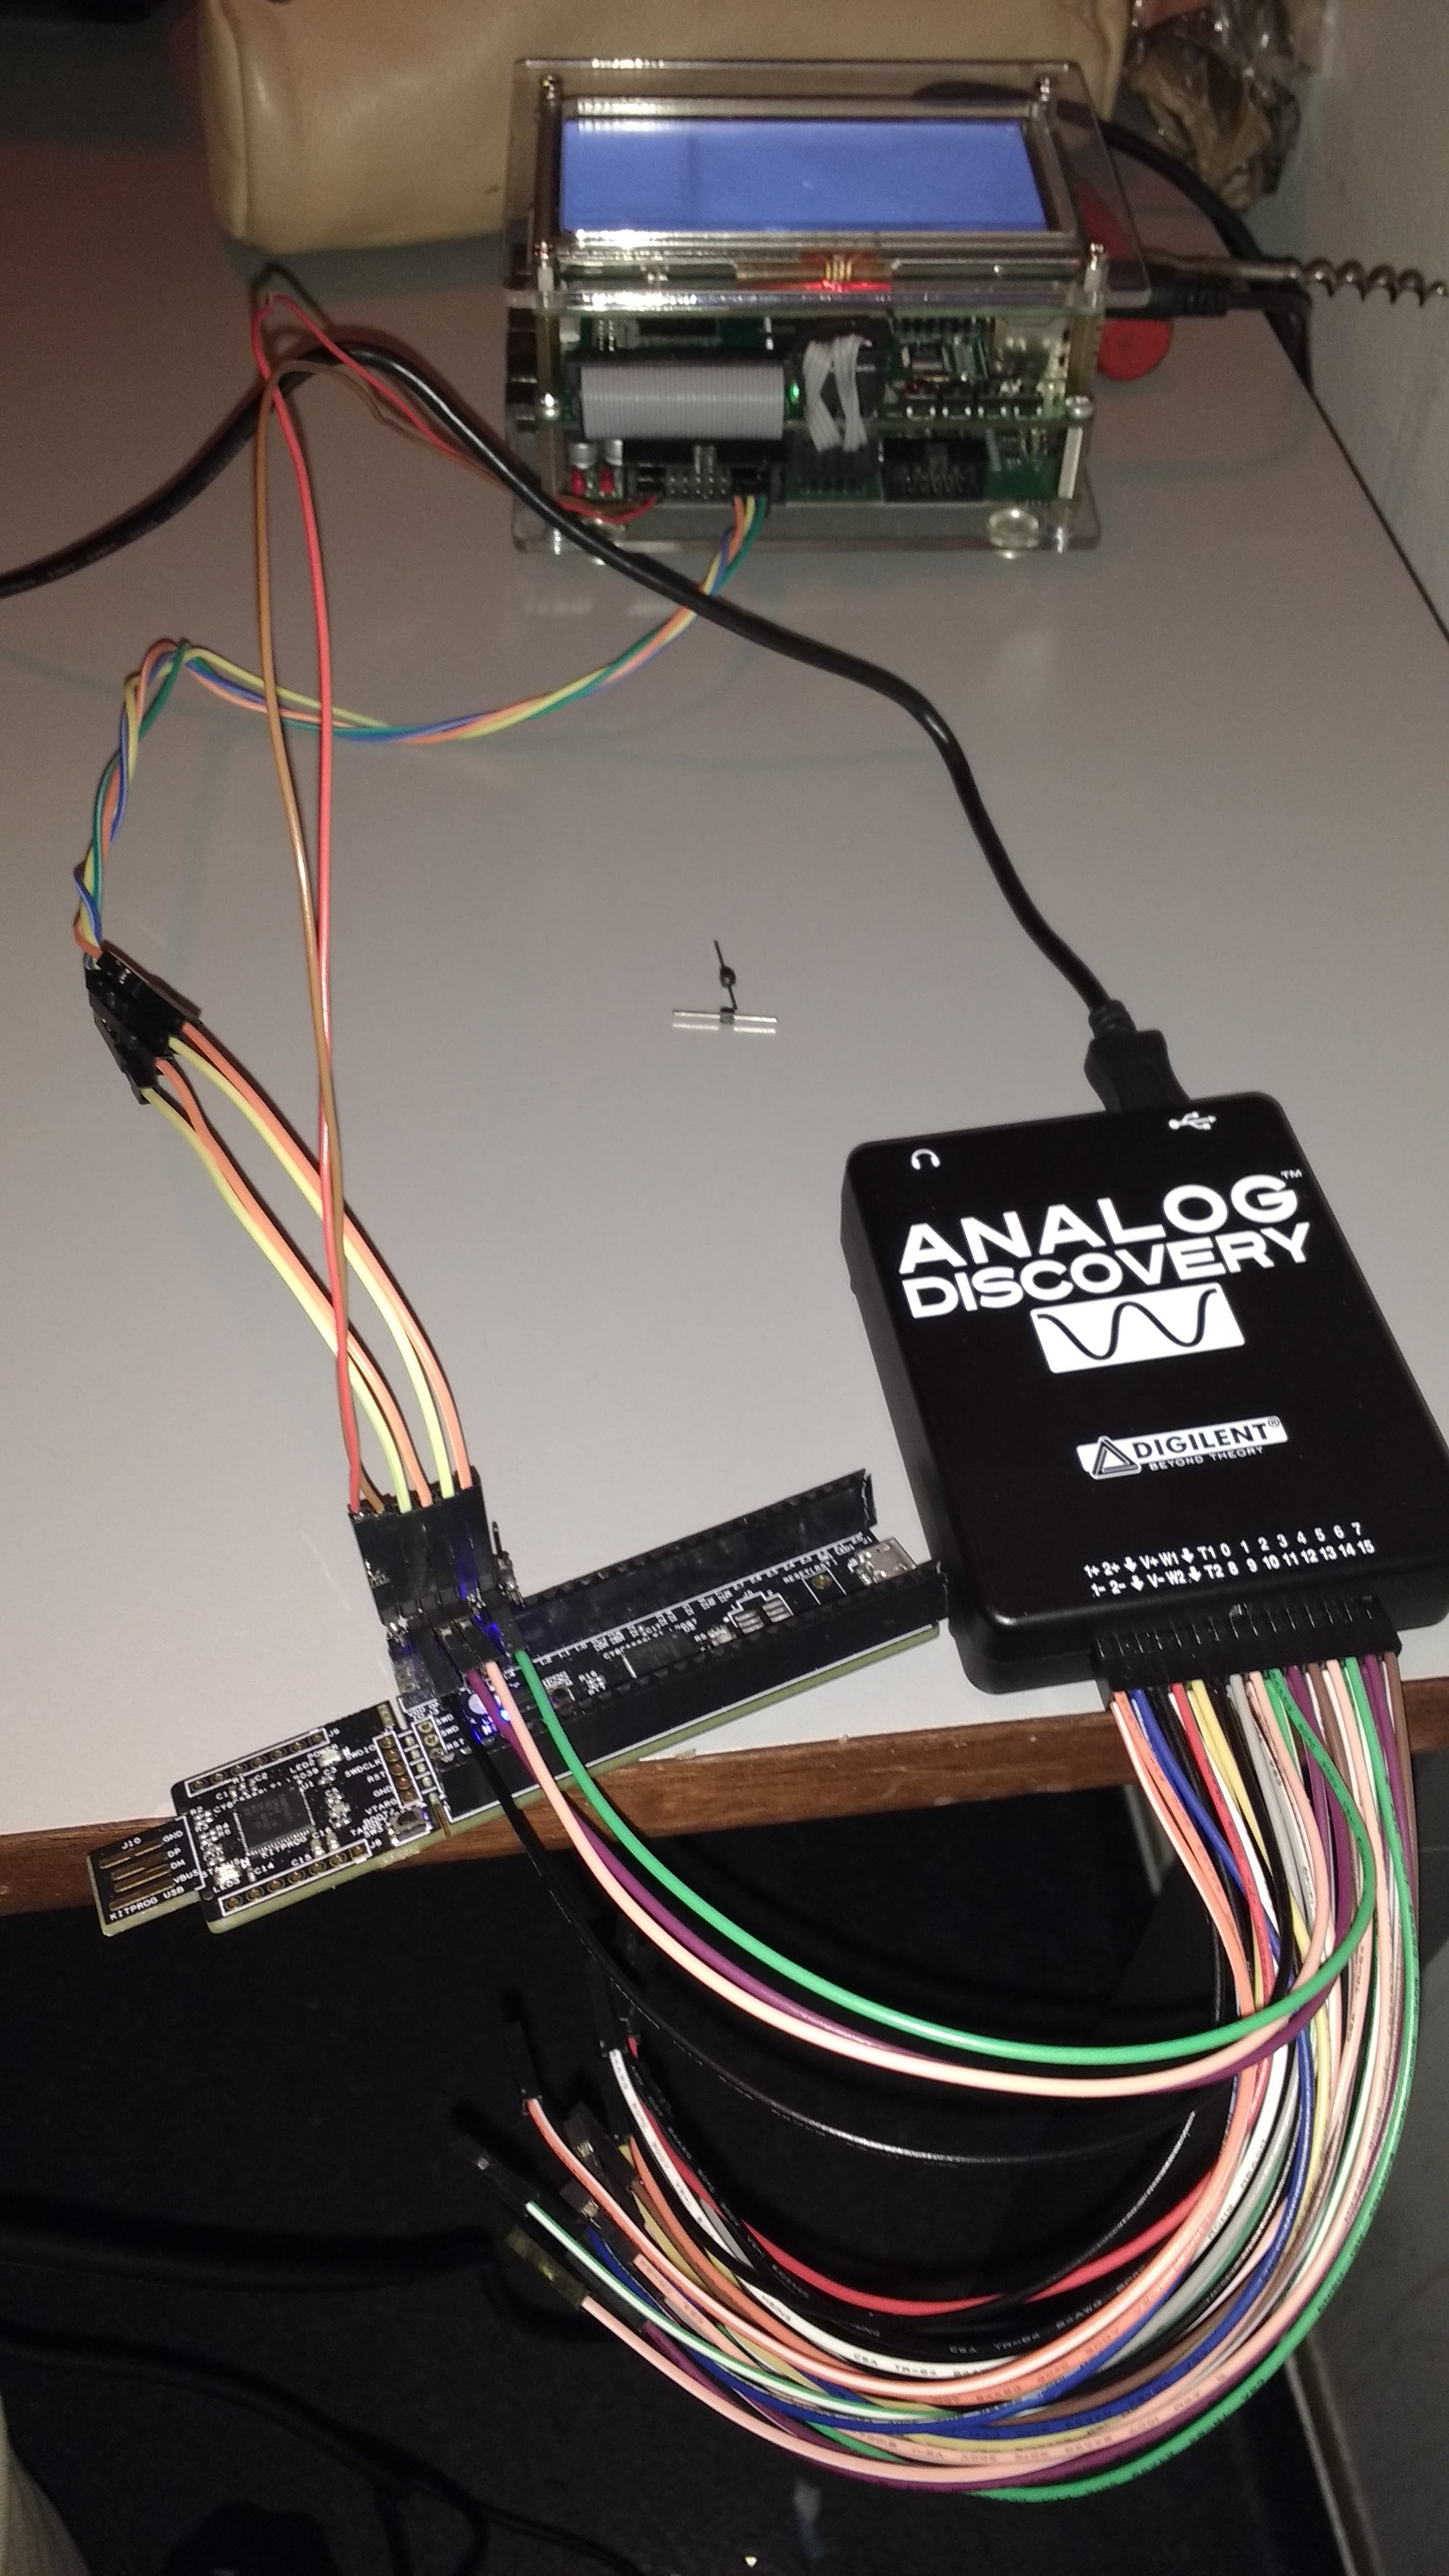
\includegraphics{Screenshots/Test_analog}
\caption{Opstilling med analog discovery til test af SPI forbindelse} 
\end{figure}

Der udføres to test scenarier. I første test sendes data fra Devit8000(master) og der foretages en måling på MOSI forbindelsen med logic analyzer
funktionen på analog discovery. Denne test skal sikre at vi får sendt de korrekte adresse og data bits over til PSoC1, samt at SS og CLCK opfører sig 
som ønsket. Det vil sige at SS går lav ved dataoverførsel og at CLCK er stabil. I denne test bruges linux terminalen på devkit8000 til at sende nogle forskellige
værdier til PSoC1 med linux kommandoen echo, hvorefter der aflæses bit kombinationer på logic analyzer.

I anden test læses der fortsat på MOSI forbindelsen, og linux kommandoen cat bruges til at læse fra PSoC1. Her aflæses det på terminalen hvad der bliver sendt 
fra PSoC1. I test programmet på PSoC1 er der implementeret en switch, som gør at når der læses med kommandoen cat PSoC{\_}5 fra devkit terminalen, vil 
status på knap 2.1 på PSoC1 blive aflæst. Således kan det testes at der sendes den korrekte data fra MISO.     


\section{Resultater}
\subsection{Resultater af test for Devkit-PSoC SPI}
Ved første test scenarie ses hvordan der sendes værdien 20 fra devkit til PSoC1 med linux kommandoen echo. På logic analyzer ses at der sendes to gange 8bit.
først en adresse kode, som er 65, og derefter værdien 20. Det ses også at SS går lav ved dataoverførelse og at clock er stabil. Testen er derfor tilfredsstillende.
 
\begin{figure}[H]
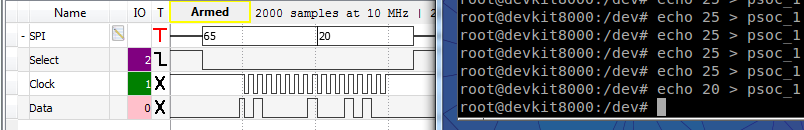
\includegraphics{Screenshots/Analog_devkit_echo_psoc_1}
\caption{Data bliver sendt fra Devit8000 til PSoC1} 
\end{figure}

Ved anden test scenarie bruges linux kommandoen cat til at læse fra PSoC1. Her ses at der sendes en adresse bit 5 og 0 via MOSI, og på terminalen ses
status for knappen på PSoC1, som er trykket nede og derfor viser 1. 

\begin{figure}[H]
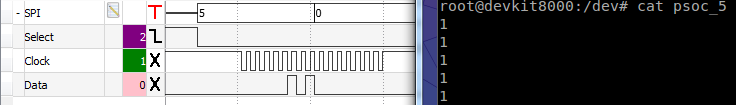
\includegraphics{Screenshots/Analog_cat_psoc_5}
\caption{Data bliver læst fra PSoC1} 
\end{figure}

\section{Diskussion}
Ud fra ovenstående ses det at SPI kan bruges til at kommunikere imellem devkit8000 og PSoC1, samt at kommunikere imellem PSoC enhederne. Som resultaterne af 
testen viser er SPI en smart måde hvorpå der kan sendes og modtages data samtidigt. Det skal dog nævnes at der har været mange problemer med denne kommunikation,
og der er brugt adskillige timer på at få det til at virke. Så sammenlignet med UART som fungerede problemfrit på 1 og 2 semester, så har SPI været meget mere
udfordrene at få til at virke. 